\chapter{The Deeplearning4j Library}

Deeplearning4j is an open-source, distributed, deep learning library for Java and Scala. Integrated with Hadoop and Spark, DL4J is specifically designed to run in business environments on distributed GPUs and CPUs.

\section{Architecture of the library}
The library is composed by several sub-libraries:

\begin{description}[leftmargin=!,labelwidth=\widthof{\bfseries Deeplearning4j}]
	\item [Deeplearning4j] provides the tools to implement neural networks and build computation graphs
	\item [Nd4j] is the mathematical back-end of Deeplearning4j. It provides the data structures for the n-dimensional arrays and allow Java to access the native libraries via JavaCPP and the Java Native Interface.
	\item [Libnd4j] is the computing library that provides native operations on CPU and GPU. It's written in C++ and Cuda.
	\item [Datavec] provides the operations for the data processing such that data ingestion, normalization and transformation into feature vectors.
\end{description}


\section{The Importance of Nd4j in the Library}
\label{sec:nd4jBlas}

Nd4j (N-Dimensional Arrays for Java) is at the base of the Deeplearning4j library, it provides data storage, manipulations, and operations. It gives the atomic pieces needed to build more complex deep learning systems. It is a scientific computing library for the JVM.  It exposes n-dimensional arrays that can be used in linear algebra and large-scale matrix manipulation. It supports CPU and GPU computations through interchangeable backends. The different backends use the same interface: they can be swapped without any change to the implementation code.

The APIs provided by the library are essentially wrappers for the different version of BLAS (Basic Linear Algebra Subprogram). 

BLAS is a specification that defines the low-level routines for linear algebra operations (for vectors and matrices). There exist several libraries implementing those subroutines in C or Fortran for dense or sparse formats. In Nd4j the BLAS subroutines can directly be called from Java thanks to JavaCPP, that internally uses the Java Native Interface (JNI) to call native routines from the JVM environment. This architecture allows the library to benefit from the advantages of the native side.

\begin{figure}[h]
	\begin{center}
		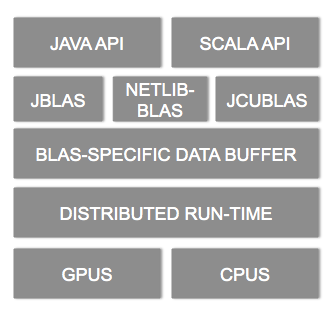
\includegraphics[width=2.5in]{images/nd4j_architecture.png} 
		\label{fig:hierachy}
		\caption{Nd4j architecture}
	\end{center}
\end{figure}

\section{Nd4j Needs a Sparse Representation}

In Deeplearning4j, Sparse Data is treated as dense and use the dense operations of BLAS and Libnd4j to perform computations. With a new sparse representation, we can gain in storage space and computation speed.

Currently, there is no library in the JVM ecosystem that provides the sparse representations and the accelerated operations. For example, Breeze library \cite{breeze} does support the sparse vectors and the sparse CSR matrices but does not have sparse tensor. Moreover, the operations provided by Breeze are not accelerated. 

Nd4j will be the first JVM library to support the sparse tensors with their accelerated operations.
